%% Template file for all Software/Hardware modules

\subsection{Add-Ons}
The Server provides for the computational needs of the POW\-R project, but
more hardware shall be added before the utility needs of the project are met.
% Talk about what needs to be added to the server and why

\subsubsection{IP Display}
The IP of the Server shall be displayed somewhere on it's casing. This is so that
the user can easily find the network address of the Server so that they can log in
to it.

This will be achieved by connecting an Arduino via USB to the Server, and housing it 
inside the Server's casing with it. The Arduino will be connected to an LCD display
which will output the network IP of the Server. Figure \ref{ArduinoLCD} shows
the interaction between Server and Arduino.

\begin{figure}
\centering
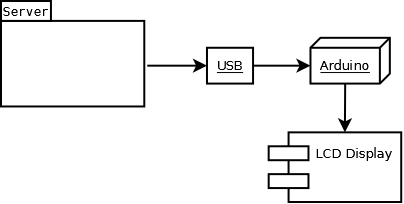
\includegraphics[scale=0.5]{Hardware/images/ArduinoLCD.png}
\caption{IP Display Diagram}
\label{ArduinoLCD}
\end{figure}

The IP of the system can be obtained via kernel module, and sent to the Arduino
one byte at a time. This works well, since the Arduino connects over serial and
thusly takes a bite at a time.


\subsection{GPIO Pins}

\subsubsection{Power Switch}

\subsubsection{Factory Reset}

\subsubsection{Connect to Satellite}

\subsection{Server Hull}

% Explain that the server needs some kind of
% legit casing, which covers all unnecessary
% ports. It must also have holes for the above
% hardware.

